\documentclass[a4paper, 12pt]{article}
\usepackage[latin1, utf8]{inputenc}
\usepackage{graphicx}
\usepackage[francais]{babel}
%\usepackage[english,french]{babel}
\usepackage{amsmath}
\usepackage{amssymb}
\usepackage{mathrsfs}
\usepackage{multicol}
\usepackage{xcolor}
\usepackage[top=2.5cm, bottom=2.5cm, left=2cm, right=2cm]{geometry}
\usepackage{fancyhdr}
\lhead{\bsc{CE321}}
\rhead{\bsc{Challenge Entreprise}}
\renewcommand{\headrulewidth}{1px}
\lfoot{ \bsc{Enseirb-Matmeca}}
\rfoot{ \bsc{I3 - Robot}}
\renewcommand{\footrulewidth}{1px}
\pagestyle{fancy}
\usepackage[colorlinks=true,linkcolor=black,urlcolor=blue]{hyperref}
\usepackage{soul}
%\usepackage{wrapfig}
%\usepackage{framed}
%\usepackage[vlined,lined,boxed,french,longend]{algorithm2e}


%%%%%%%%%%%%%%%% Variables %%%%%%%%%%%%%%%%
\def\projet{Rapport d'activité}
\def\titre{ArchMobile}
%\def\groupe{2}
%\def\equipe{4}
%\def\responsible{classerre}
%\def\secretary{ahavlicek}
\def\others{Hofer, Lambert, Lasserre, Le clec'h}

\graphicspath{{graphics}{data/}}

\begin{document}
%%%%%%%%%%%%%%%% Header %%%%%%%%%%%%%%%%
\begin{center}
\vspace*{10mm}
\Huge{\bfseries \sffamily \projet}
\vskip 20mm
\huge{ \itshape \titre}
\vskip 10mm
\huge{ \sffamily \others}
\vskip 5mm
\end{center}


\vskip 15mm
\begin{minipage}{.49\textwidth}
  
\includegraphics[width=\linewidth]{flyer}
\end{minipage}
\begin{minipage}{.49\textwidth}
  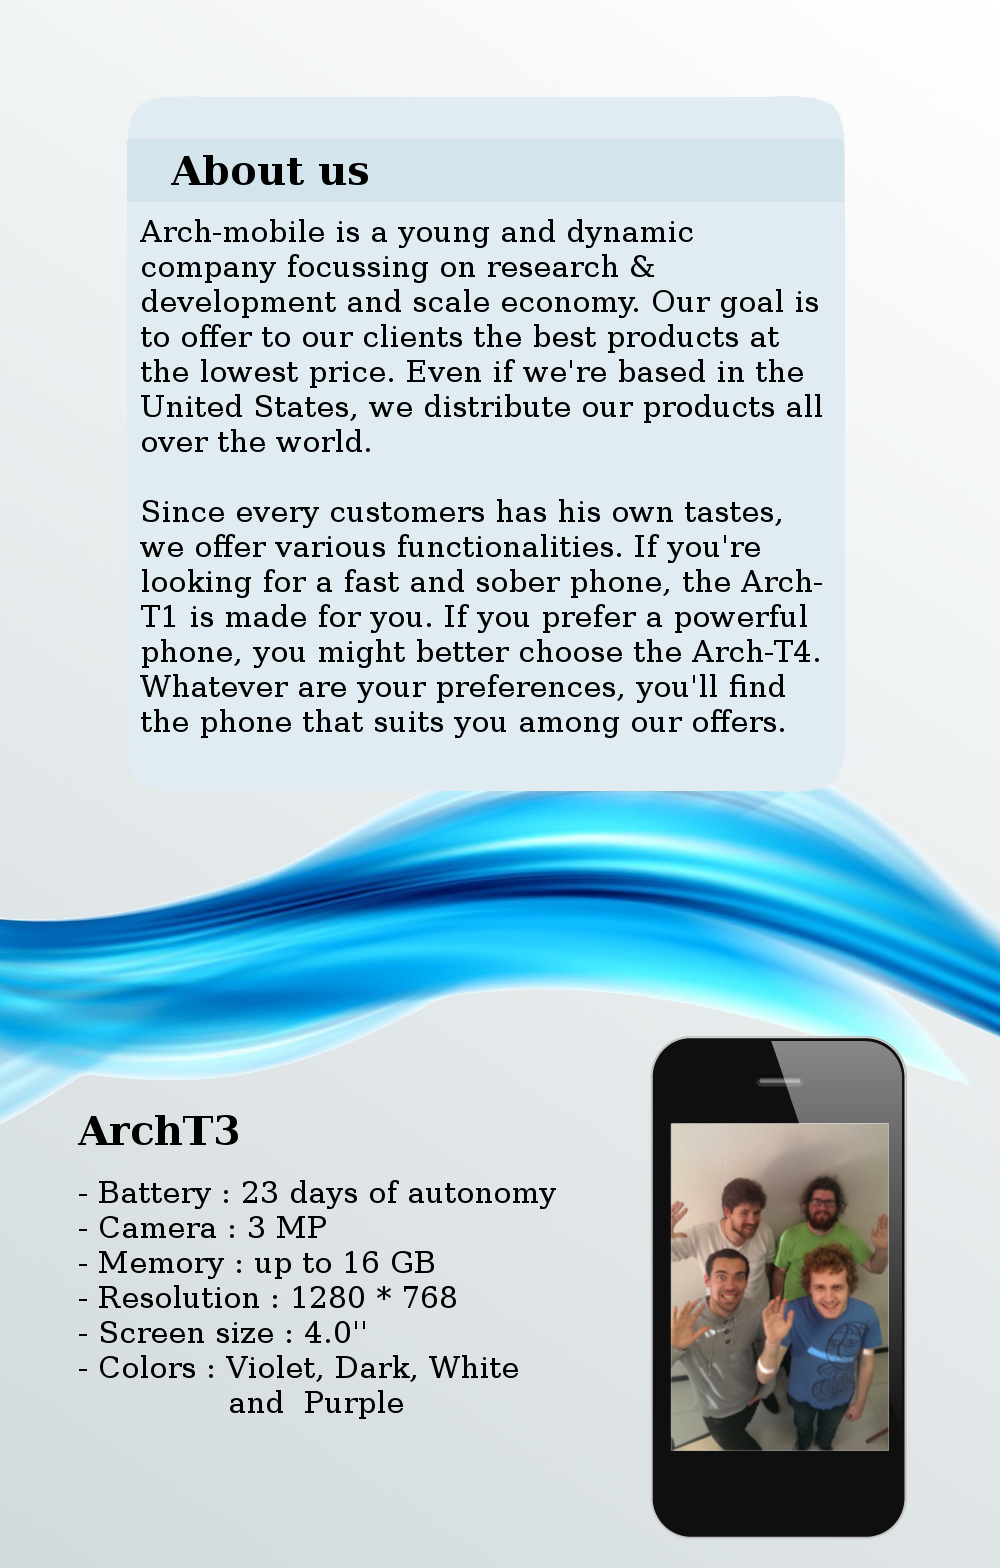
\includegraphics[width=\linewidth]{flyerVerso}
\end{minipage}

\vskip 30mm

\pagebreak

%%%%%%%%%%%%%%%% Main part %%%%%%%%%%%%%%%%

\section{Introduction}
\subsection{Membres de l'équipe}
\begin{itemize}
\item Ludovic Hofer
\item Thibault Lambert
\item Christian Lasserre
\item Louis Le Clec'h
\end{itemize}


\subsection{Lettre aux Actionnaires}
Cher actionnaires,\\

\begin{minipage}[t]{0.45\textwidth}
\paragraph{} L'année 2013 touche à sa fin, notre groupe a atteint les objectifs qu'il s'était fixés.
	 Nous devons ces résultats à l'ensemble de nos salariés qui ont oeuvré pour la réussite de l'entreprise.
	 Malgré les difficultés lié à une concurrence toujours plus intense, notre groupe a su conserver une image de qualité.
	 La réussite d'une entreprise comme la nôtre passe par un juste équilibre entre ses parties prenantes: salariés, clients et actionnaires.
	 Vous êtes en effet essentiels pour l’entreprise, car votre fidélité concourt à sa pérennité et à son développement. 

\end{minipage}
\hfill
\hspace*{0.1\textwidth}
\begin{minipage}[t]{0.45\textwidth}
\paragraph{} Le chiffre d'affaire a subit une légère baisse cependant le résultat opérationnel global du groupe est remonté.
	 Notre politique de qualité a porté ses fruit en Europe et nous a permis d'augmenter notre EBITDA de plus de 20\%.
	 Les bons résultats de notre groupe ont permis de nouveau d'augmenter la valeur de nos actions.\\

\paragraph{} J’espère, cher actionnaire, que la performance de votre Groupe et ses perspectives d’avenir sont à la hauteur de vos attentes.
	 Je vous remercie de votre fidélité.
\end{minipage}




\subsection{Présentation de ArchMobile}
Multinationale Américaine de téléphonie mobile, Archlinux 
est rapidement devenu un des leader de son domaine.
Devenu le premier constructeur mondial de téléphonie mobiles 
en 2013\footnote{classement établi par M. Eric ASTIEN},
ArchMobile s'est illustré sur ces 5 dernières années par
la confiance qu'il a su établir au sein d'une clientelle 
de qualité. Malgré un essai peu concluant dans le low-cost,
leurs produits atteigne désormais une qualité, un apport
technologique et une fiabilité inégalé sur l'ensemble du
marché.



\paragraph{\'Etymologie}~\\
Le nom ``ArchMobile'' provient de la distribution ``ArchLinux'' sur
laquelle est bâtie le téléphone. L'hypothèse la plus plausible est que
les fondateurs de la société se soient inspiré du premier nom qu'ils
aient entendu. 

\paragraph{Produits}~\\
ArchMobile s'est imposé progressivement sur le marché avec 3 technologies:
\begin{itemize}
\item ArchT1 : incluant la Tech1, sortie rapidement sur le marché et qui a assuré 
  des revenus réguliers sur les premières années de la compagnie.
\item ArchT3 : produit phare, sortie après une période de disette 
  économique et fruit de gros efforts de la société à long terme.
\item ArchT4 : le dernier produit high-tech de ArchMobile qui assoit
  sa différenciation par le haut sur le marché.
\end{itemize}

\paragraph{Valeurs}
\subparagraph{Ecologie}
Depuis toujours, Archmobile concilie écologie, responsabilité et
design. Tous nos composant sortent d'usine certifiée MAX HAVELAAR, et
tout nos employés ont a coeur la conservation de notre planète.
\subparagraph{Entraide}
Archmobile s'engage également régulièrement au côté d'association
caritative, et à créer sa propre fondation ``les orphelins de
l'Arche'' qui aide des enfants victimes de la guerre a retrouver un
foyer.
\subparagraph{Art}
Archmobile aime les arts et le prouve en organisant tout les ans le
festival du cinémé d'art et d'essai de Guingamp, ainsi que le festival
de danse colombienne ancienne de Montauban.
\subparagraph{Science}
Depuis deux ans, Archmobile soutient l'association d'aide au mythomane
(l'AAM) en lui permettant d'approcher des homme politiques de tout
bords.


\pagebreak

\section{PARTIE 1 : EXAMEN DE LA STRATÉGIE}
\paragraph{Première année sous notre direction}
Notre strategie était basée sur l'évolution de l'implémentation des
antennes dans les diverses zones géographiques. Nous voulions jouer
sur la montée en puissance de la tech 3 en asie puis aux états-unis,
tout en gardant une base de vente régulière avec la tech 1. Pour cela
nous avons d'emblé fait des investissements lourds dès la première
année, en achetant dix nouvelles usines en Asie, en embauchant
massivement des ingénieurs, en augmentant de 600 à 1500 dollars le
budget de la formation par ingénieur, et en augmentant les salaires
des ingénieurs a 5000 dollars par mois.

\paragraph{La crise des télécoms:}

Ce choix, bien qu'il se soit révélé payant, à été compliqué à gérer
notamment durant la troisième année, première année de la dure crise
qui a touché le secteur des télécoms. En effet les perspectives
étaient plutôt sombres, nos concurrents faisaient de bon chiffres sur
la tech 2, nos ventes de télephone tech 1 commençait à s'essouffler et
le marché n'était pas prêt à acceuillir la tech 3. Nous avons donc
décidé de prendre un minimum de risque sur ce tour, en diminuant notre
production et en tatant le terrain en Asie avec la tech 3. Nous avons
également émis un certain nombre d'action pour pouvoir racheter nos
dettes et diminuer le poids des interets sur nos résultats.

\paragraph{La reprise:}

La quatrième année à été tournant pour notre compagnie. Alors que nos
concurrents ont accumulé les pertes, nous avons eu une bonne année, en
prenant 3\% de part de marché global et en ayant des pertes très
mesurées. Notre compagnie representait près de 24\% du marché
asiatique, très loin devant la plupart de nos concurrents.

\paragraph{L'envolée:}

Notre compagnie a commencée a réelement prendre son envol durant la cinquième année. nos capacité de production importante ainsi que notre R\&D efficace nous a permis de sortir de meilleurs téléphones (introducton de la tech 4 en europe) et d'améliorer nos marges. On observe aussi que notre chiffre d'affaire est superieur de 30\% a celui de la majorité de nos concurrents. Devant la montée en puissance de la capacité de production de nos concurrents, nous avons fait le choix de ne pas augmenter notre nombre d'usine, en profitant de notre bonne santé financière pour viser un repositionnent de notre gamme de téléphone vers le haut de gamme. Ce sera notamment la dernière année ou nous produirons de la tech 1.

\paragraph{L'age d'or:}

La sixième année fut une année faste pour Archmobile. Des résultats
records et de solides bénéfices ont consacrée Archmobile comme la
première entreprise du secteur. Nous avons profités de nos liquidités
importantes pour commencer a verser des dividendes a nos actionnaires,
et à racheter des actions. Décisions est également prise de réduire la
voilure au niveau du personnel en commençant à diminuer le salaires de
nos ingénieurs, afin d'améliorer nos marges.

\paragraph{Les premières turbulances:}

La septième année a été difficile pour nous, après une excelente
sixième année, nous étions ratrappé par nos concurrent, qui avait
cassé les prix et pris nos part de marché au point que nous n'avions
jamais eu autant de stock a la fin d'un exercice (plus de quatre
millions de mobile). Notre chiffre d'affaire était également en baisse.
Malgré tout,nos bénéfices restaient confortable.

\paragraph{La reconquête:}
 
Nous avons décidés sur le huitième exercice de 



\pagebreak

\section{PARTIE 2 : EXAMEN DE LA PERFORMANCE}
\paragraph{}
La stratégie de domination par les coûts que nous avons menée dans les premiers
tours s'est révelée peu fructueuse. En effet, une majorité des autres 
entreprises sont parties sur une stratégie du même type. Cela a eu pour effet
une chute importante des prix de la technologie 1 pendant les premiers tours. 
Comme une majorité des entreprises augmentait leur puissance de production, 
le marché s'en est trouvé inondé. De plus les tours de crises n'ont fait
qu'empirer la situation en diminuant la taille du marché quand la capacité de
production globale augmentait. Suite à cette analyse, nous avons conclu qu'il 
fallait au plus vite abandonner la technologie 1: les prix étaient devenus trop 
faibles pour permettre une rentabilité financière importante.

\paragraph{}
Au terme de la compétition, nous étions la seconde entreprise avec le moins de
part de marché mais cela ne nous a pas empêché d'être ceux qui avaient le
cours de l'action en bourse le plus haut. Même aux bénéfices, nous figurions
deuxième. Ceci s'explique facilement par le fait que nous ne vendions que des
téléphones des dernières technologies, avec de nombreuse fonctionnalités.
Étant positionnés sur un marché de luxe, nous étions aptes à pratiquer des
prix élevés nous permettant ainsi de jouir de marges conséquentes. Le bénéfice
dégagé par unité de production était donc particulièrement élevé dans notre
entreprise.

\paragraph{}
Notre choix de commencer à développer assez tôt les techologies 3 et 4 a payé
puisqu'au cours de la 9ème année, nous étions parmi ceux qui avaient les coûts
de production les plus bas
\footnote{Voir figures \ref{coutTech3} et \ref{coutTech4}.}
pour ces deux technologies particulièrement prisées et rentables. Nous avons
ainsi bien profiter de l'effet d'expérience, notre choix de nous passer de la
technologie 2 semble donc avoir porté ses fruits. Il est aussi possible de
remarquer qu'une seule entreprise était réellement capable de rivaliser avec
nous sur les coûts de production de la technologie 4 (ERATEL). En revanche,
elle avait un coût de production bien plus élevé en ce qui concerne la
technologie 3. On peut donc considérer que ce qui nous a réellement permis de
nous démarquer a été notre aptitude a être compétitif de manière simultanée
sur les deux marchés les plus fructueux. De plus, nous avons pu observer qu'en
nous plaçant sur des marchés haut-de-gamme, le problème de gestion des stocks
devenait moins critique.


\begin{figure}
  \caption{\label{coutTech3}Cout de production de la technologie 3}
  \centering
  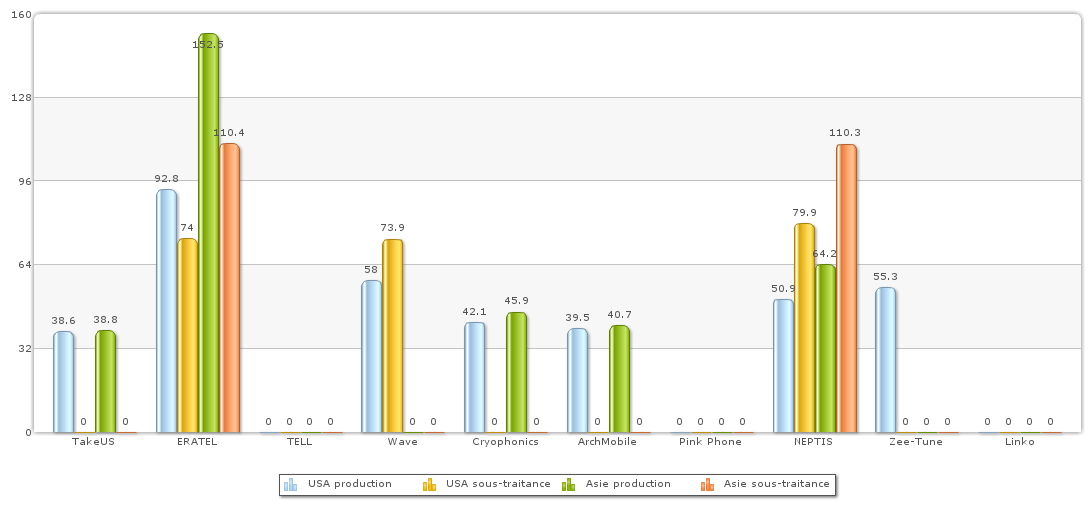
\includegraphics[width=\textwidth]{CoutTech3.png}
\end{figure}

\begin{figure}
  \caption{\label{coutTech4}Cout de production de la technologie 4}
  \centering
  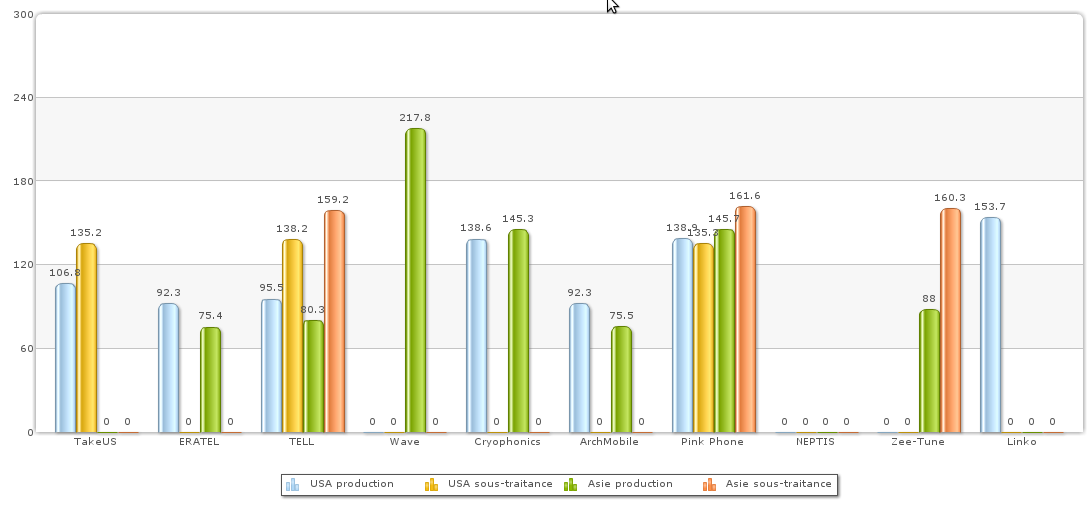
\includegraphics[width=\textwidth]{CoutTech4.png}
\end{figure}


\pagebreak
\section{CONCLUSION : ANALYSE DE LA COMPÉTITION}
% Départ difficile
\paragraph{}
Après un départ tumultueux et un classement peu gratifiant, nous avons réussi
à remonter progressivement pour finalement arriver à la première place et y
rester. Ces faibles scores sont facilement expliquables par les nombreux
investissements à long terme que nous avons effectué pendant la première
année. L'accent que nous avons mis sur la recherche nous a handicapé au début
mais nous a propulsé au sommet du classement lorsque la couverture des
différentes zones s'est améliorée.

% Succès = tête froide + travail d'équipe
\paragraph{}
Notre progression constante est principalement dûe au fait que nous avons su
nous raisonner au sein du groupe, évitant ainsi des stratégies trop risquées
qui auraient pu nous mener à la catastrophe. Nous avons réussi à éviter les
conflits en faisant souvent des compromis entre les différents points de vue.
Plusieurs fois nous nous sommes rendus compte que si nous ne nous étions pas
écouter mutuellement, nous aurions fait de grosses erreurs.

% Fin difficile
\paragraph{}
Notre montée en flèche à mi-parcours s'est progressivement ralentie et au
final, d'autres équipes étaient bien parties pour remonter l'écart s'il y
avait eu plus de tours. Cette situation est dûe au fait que la simulation ne
permettait pas de continuer la recherche après la technologie 4. La limite de
tour nous a aussi décourager d'acheter de nouvelles usines, quelque chose que
nous aurions pu nous permettre de faire s'il restait plus d'années
d'exploitation. Nous sommes donc resté pendant plusieurs exercices avec des
fonds considérables sans trouver de réelles possibilités de le réinvestir.
Nous versions donc les plus grands dividendes possibles aux actionnaires, sans
pour autant réussir à écouler nos fonds. Or, il n'y a pas de situation plus
gênante pour une entreprise que de laisser dormir son argent.

\paragraph{}
Au cours de notre session, l'offre a toujours été supérieure à la demande.
Malgré ce fait, la plupart des entreprises ont continué à produire sans faire
attention aux problèmes de stock. Contrairement à elles, nous avons très
rapidement limité notre production ou baisser nos prix drastiquement dès que
nos stocks étaient trop haut. Nous avons aussi su nous débarasser de tous nos
équipements de technologie 1 avant d'arrêter d'en produire. Cette attitude
qui nous a permis de monter sur la première marche du podium logistique a
aussi hautement contribué à notre victoire.


\end{document}
